\section{Poisson Proceess}

A \underline{Poisson process} is the continuous time analog of
``coin flipping'' (or Bernoulli) processes. This makes it a good model
for arrival processes: photons hitting a detector, packets in a network,
number of emails per hour, etc.

\begin{center}
  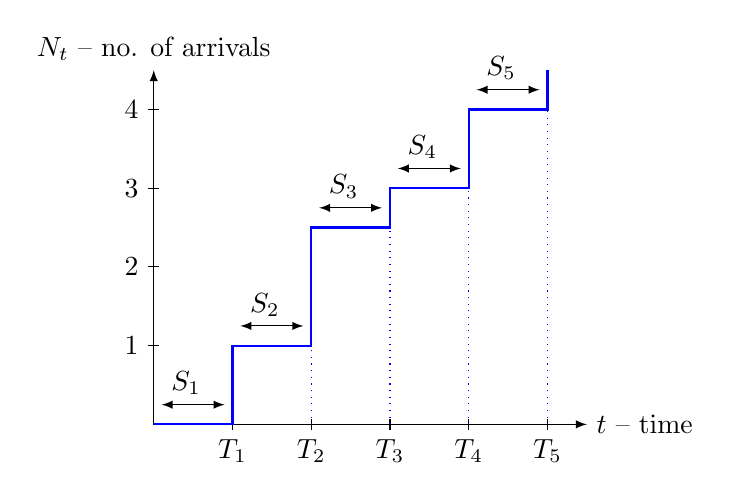
\begin{tikzpicture}[>=latex]
    \draw [<->] (0, 4.5) node [above] {$N_t$ -- no. of arrivals} |-
    (5.5, 0) node [right] {$t$ -- time};
    \foreach \x [evaluate=\x as \y using \x] in {1,...,5} \draw
    (\x,2pt) -- (\y, -2pt) node [below] {$T_{\x}$};
    \foreach \x [evaluate=\x as \y using \x] in {1,...,4} \draw
    (2pt,\x) -- (-2pt, \y) node [left] {\x};
    \draw [blue,thick] (0,0) -| (1,1) -| (2,2.5) -| (3,3) -| (4,4) -| (5,4.5);
    \draw [blue,dotted] (2,0) -- (2,1);
    \draw [blue,dotted] (3,0) -- (3,2.5);
    \draw [blue,dotted] (4,0) -- (4,3);
    \draw [blue,dotted] (5,0) -- (5,4);
    \draw [<->] (0.1,0.25) node [above right] {$S_1$} -- (0.9,0.25);
    \draw [<->] (1.1,1.25) node [above right] {$S_2$} -- (1.9,1.25);
    \draw [<->] (2.1,2.75) node [above right] {$S_3$} -- (2.9,2.75);
    \draw [<->] (3.1,3.25) node [above right] {$S_4$} -- (3.9,3.25);
    \draw [<->] (4.1,4.25) node [above right] {$S_5$} -- (4.9,4.25);
  \end{tikzpicture}
\end{center}

Each $T_i$ for $i = 1,2,3,4,5$ represents an arrival and generally,
each arrival time is defined as

\begin{displaymath}
  T_n = \sum_{i=1}^{n} S_i
\end{displaymath}

where the interarrival times
$S_1,S_2,\ldots,S_n \overset{\textrm{iid}}{\sim} Exponential(\lambda)$.
Thus, every $S_i$ has the probability density function

\begin{displaymath}
  f_{S_i}(t) = \lambda e^{\lambda t};\ t > 0;\quad i=1,2,3,\ldots
\end{displaymath}

and cumulative distribution function

\begin{displaymath}
  F_{S_i}(t) = 1 - e^{-\lambda t};\quad i = 1,2,3,\ldots
  .
\end{displaymath}

\begin{definition}[Number of Arrivals]

  \begin{displaymath}
    N_t =
    \begin{cases}
      \max_{n \geq 1} \{n \mid T_n \leq t\} & t \geq 0 \\
      0 & t < T_1
    \end{cases}
  \end{displaymath}

\end{definition}

\begin{itemize}
  \item Recall: $Exponential(\lambda)$ is a memoryless RV
    \begin{enumerate}
      \item $F_{\tau}(t) =
        \begin{cases}
          1 - e^{-\lambda t} & t \geq 0 \\
          0 & t < 0
        \end{cases} \Rightarrow f_{\tau}(t) = \lambda e^{-\lambda t}$
      \item $\E\left[\tau\right] = \frac{1}{\lambda}$ and $\Var(\tau)
        = \frac{1}{\lambda^2}$
      \item $\Prb(\tau > t + s \mid \tau > s) = \Prb(\tau > t)$
      \item $\Prb(\tau \leq t + \epsilon \mid \tau > t) = \lambda
        \epsilon +o(\epsilon);\ \lim_{\epsilon \rightarrow 0}
        \frac{o(\epsilon)}{\epsilon} = 0$
    \end{enumerate}
\end{itemize}

\begin{proof}

  \begin{align*}
    \Prb(\tau > t + \epsilon \mid \tau > t) &= \Prb(\tau > \epsilon) \\
    &= e^{-\lambda \epsilon} \\
    &= 1 - \lambda \epsilon + o(\epsilon) \\
    \therefore \Prb(\tau \leq t + \epsilon \mid \tau > t ) &= 1 - \Prb(\tau
    > t + \epsilon \mid \tau > t) \\
    \lambda \epsilon + o(\epsilon)
  \end{align*}

\end{proof}

\begin{itemize}
  \item $\Prb(\text{1 arrival}) = \lambda \epsilon + o(\epsilon)$
  \item $\Prb(\text{2 arrivals}) = 1 - \lambda \epsilon + o(\epsilon)$
  \item $\Prb(\text{3 arrivals}) = o(\epsilon)$
\end{itemize}

We can only have one arrival in a particular subinterval with high
probability $\lambda \epsilon + o(\epsilon)$. On the other hand,
there are zero arrivals with probability
$1 - \lambda \epsilon + o(\epsilon)$.

This means that a Poisson process has \underline{independent} and
\underline{stationary} increments, i.e., for any
$0 \leq t_1 \le t_2 \le \ldots \le t_n \le \ldots$; if you look at the
number of arrivals in $t_{n+1}$ and $t_n$, $\{N_{t_{n+1}} - N_{t_{n}}\}$
are independent and the distribution depends only on the size of the
interval $(t_{n+1} - t_n)$.

\begin{theorem}
  Let $N_t \coloneq$ number of arrivals in $(0,t)$, then
  \begin{displaymath}
    P(N_t = k) = e^{-\lambda t} \frac{(\lambda t)^k}{k!};\quad k = 0,1,2,\ldots
  \end{displaymath}
  \begin{proof}

    \begin{displaymath}
      P(N_t = k) = \int_{t_1} \int_{t_2} \ldots \int_{t_k}
      f_{T_1,T_2,\ldots,T_k \mid N_t = k}(t_1,t_2,\ldots,t_k \mid N_t
      = k) dt_1\ dt_2\ \ldots\ dt_k
    \end{displaymath}

    We constrain the region of integration by letting
    $S = 0 \le t_1 \le t_2 \le \ldots \le t_k \le t \le t_{k+1}$.
    Shifting focus to the $k^{\text{th}}$ dimensional pdf,

    \begin{displaymath}
      f_{T_1,\ldots,T_k \mid N_t = k}(t_1,\ldots,t_k \mid N_t = k) =
      \Prb(T_1 \in (t_1,t_1 + dt_1),\ldots,T_k \in (t_k,t_k + dt_k),T_{k+1} > t)
    \end{displaymath}

    where we leverage the fact that
    $\Prb(T_{k+1} \in (t_{k+1}, t)) = \Prb(T_{k+1} > t)$

    \begin{align*}
      &\Rightarrow \Prb(T_1 \in (t_1,t_1 + dt_1)) \times \ldots
      \times \Prb(T_k \in (t_k,t_k + dt_k)) \times \Prb(T_{k+1} > t) \\
      &= \Prb(S_1 \in (t_1,t_1 + dt_1)) \times \ldots \times \Prb(S_k
      \in (t_k - t_{k-1},t_k - t_{k-1} + dt_k)) \times \Prb(S_{k+1} >
      t - t_k) \\
      &= (\lambda e^{-\lambda t_1} dt_1)\ \ldots\ (\lambda
      e^{-\lambda (t_k - t_{k-1})} dt_k)\ e^{-\lambda (t - t_{k})} \\
      &= \lambda^k e^{-\lambda t}
    \end{align*}

    The result $\lambda^k e^{-\lambda t}$ is a constant to the
    $k^{\text{th}}$ dimensional integral, so barring any constraints on
    $t_1,t_2,\ldots,t_k$, $\textrm{Volume}\ (S) = t^k$. But, we must
    respect the fact that $0 \le t_1 \le t_2 \le \ldots \le t_k$.

    By symmetry, every permutation of $(t_1,t_2,\ldots,t_k)$ has
    equal volume

    \begin{displaymath}
      \textrm{Volume}\ (S) = \frac{t^k}{k!} \Rightarrow \Prb(N_t = k)
      = \frac{(\lambda t)^k e^{-\lambda t}}{k!}; \quad k=0,1,2,\ldots
    \end{displaymath}

  \end{proof}

  \begin{itemize}
    \item Conditioned on the number of arrivals being $k$ in an
      interval, the density is uniform
    \item Intuition behind symmetry argument: $k=2$
      \begin{center}
        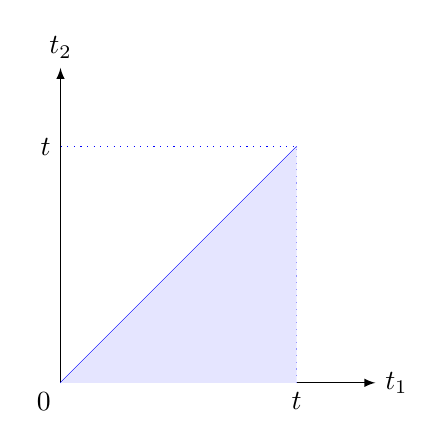
\begin{tikzpicture}[>=latex]
          \draw [<->] (0, 4) node [above] {$t_2$} |-
          (4, 0) node [right] {$t_1$};
          \draw (0,0) node [below left] {$0$};
          \draw (0,3) node [left] {$t$};
          \draw (3,0) node [below] {$t$};
          \draw [blue] (0,0) -- (3,3);
          \draw [blue,dotted] (3,0) -- (3,3);
          \draw [blue,dotted] (0,3) -- (3,3);
          \fill [blue!10] (0,0) -- (3,0) -- (3,3) -- cycle;
        \end{tikzpicture}
      \end{center}
      From the image above we know that
      $\Prb(t_1 \le t_2) + \Prb(t_2 < t_1) = 1$. Thus,
      $\Prb(t_1 < t_2) = \frac{1}{2} = \frac{1}{2!}$ which generalizes
      to $k$ dimensions.
  \end{itemize}

\end{theorem}

\begin{definition}[Poisson Merging]
  Merging two or more independent Poisson processes yields
  $PP(\lambda_1 + \lambda_2 + \ldots + \lambda_n)$
\end{definition}

\begin{definition}[Poisson Splitting]
  Let $N \sim PP(\lambda)$ such that $N$ is split into $N_1$ and $N_2$.
  For each arrival we flip a coin independently with probability
  $H = p$. If the coin lands on heads, send the arrival to the $N_1$
  queue otherwise it is sent to the $N_2$ queue.
\end{definition}
